\documentclass[11pt]{article}
\usepackage[margin=1in]{geometry}
\usepackage{amsmath,amssymb}
\usepackage{booktabs}
\usepackage{siunitx}
\usepackage{hyperref}
\usepackage{graphicx}
\usepackage{epstopdf}
\usepackage{caption}
\usepackage{xcolor}
\usepackage{array}

\sisetup{
  separate-uncertainty = true,
  per-mode = symbol,
}

\title{W9: COSY Longitudinal Study --- 0.5\,ps vs 2\,ps}
\author{Eremey Valetov}
\date{25 February 2026}

\begin{document}
\maketitle

\section{Objective}

The 11-stage transverse Twiss optimisation produces identical quad currents
for both the 0.5\,ps and 2\,ps operating modes of the UH MkV FEL, as shown
analytically in S9 and numerically with FELsim.  A reviewer requests
COSY~INFINITY-level evidence that the full 3D (6D phase space) simulation
confirms this, and that the longitudinal beam quality is preserved through
the transport line.

This study uses COSY~INFINITY's differential algebra (DA) framework to
extract the complete 6D transfer map at the undulator entrance, propagate
$10^4$-particle bunches through it for both operating modes, and test
whether adding longitudinal FIT objectives changes the optimised solution.


\section{Method}

\subsection{COSY 6D Transfer Map Extraction}

The 11-stage COSY FIT optimisation is run with the standard transverse
objectives (\S\ref{sec:results-map}) and the following COSY parameters:
\begin{itemize}
  \item Computation order: 3 (DA polynomials up to 3rd order)
  \item Dimensions: 3 (6D phase space: $x, a, y, b, l, \delta$
    where $a = x'$, $b = y'$, $\delta = \delta_K = \Delta K/K_0$)
  \item Transfer matrix output order: 2 (linear + $(l|\delta\delta)$)
  \item Fringe field order: 0
  \item $E = \SI{40}{MeV}$, $\varepsilon_n = 8\;\pi\cdot\text{mm}\cdot\text{mrad}$
\end{itemize}

The full $6\times6$ linear transfer map~$\mathcal{M}$ and second-order
coefficient $(l|\delta\delta) = \text{ME}(5,66)$ are extracted via the COSY
\texttt{PM} command.

\paragraph{COSY \texttt{PM} output and $(\delta|\delta)$.}
COSY's \texttt{PM} command outputs five map components per line
(for $x, a, y, b, l$), not six: the sixth coordinate
$\delta$ is the DA independent variable, and its map is the identity by
construction in a passive beamline.  The six-digit indices (e.g.,
\texttt{000001}) confirm that the simulation uses three DA dimensions
(6D phase space), not two.  The reader code pads the missing sixth
component with zero, yielding $(\delta|\delta) = 0$ in the raw output.  We
set $(\delta|\delta) = 1$ when constructing the full $6\times6$ matrix,
consistent with energy conservation.

Evidence that the simulation is 3D, not 2D:
\begin{itemize}
  \item Six-digit polynomial indices (\texttt{dimensions=2} uses four digits)
  \item $(l|x) = 9.87\times10^{-3}$, $(l|a) = -4.80\times10^{-2}$ (non-zero
        path-length coupling through dipoles)
  \item $(l|\delta) = \SI{27.09}{mm}$ (non-zero momentum compaction)
\end{itemize}

\subsection{6D Bunch Propagation}

Gaussian bunches ($N = 10{,}000$, seed = 42) are generated in COSY
coordinates for four scenarios:
\begin{enumerate}
  \item 0.5\,ps, $h = 0$ (no chirp)
  \item 0.5\,ps, $h = 5\times10^9$\,s$^{-1}$
  \item 2\,ps, $h = 0$
  \item 2\,ps, $h = 5\times10^9$\,s$^{-1}$
\end{enumerate}
where $h$ is the linear energy chirp rate: $\delta \to \delta + h\,l/(\beta c)$.
Each bunch is propagated through the linear map:
$\mathbf{X}_\text{out} = \mathcal{M}\,\mathbf{X}_\text{in}$, with $(l|\delta\delta)$
correction applied if non-zero.

Beam parameters: $\sigma_x = \sigma_y = \SI{0.8}{mm}$,
$\sigma_{x'} = \sigma_{y'} = \varepsilon_\text{geom}/\sigma_x$,
$\sigma_\delta = 0.5\%$.

\subsection{$(l|\delta)$ Objective Test}

Two COSY FIT runs are compared:
\begin{description}
  \item[Baseline] Standard 11-stage transverse-only objectives.
  \item[Augmented] Same objectives plus $(l|\delta) = 0$ at the undulator
    entrance (element~117), using COSY's \texttt{ME(5,6)} function with
    unit weight.
\end{description}


\section{Results}

\subsection{Transfer Map Analysis}
\label{sec:results-map}

The transverse optimisation achieves $\text{MSE} = 2.27\times10^{-7}$,
matching all four Twiss targets to better than $10^{-3}$.
Table~\ref{tab:map} lists the longitudinal map elements at the undulator
entrance.

\begin{table}[ht]
\centering
\caption{Longitudinal elements of the COSY transfer map $\mathcal{M}$ at the
  undulator entrance ($E = \SI{40}{MeV}$, FR\,0, order~3).  COSY notation
  $(y_i|y_j)$ denotes the first-order map coefficient; the transport-code
  equivalents ($R_{ij}$, $T_{ijk}$) are given for reference.}
\label{tab:map}
\begin{tabular}{@{} l l l S[table-format=+1.4e-1] l @{}}
\toprule
{Map element} & {FOX} & {Transport} & {Value} & {Interpretation} \\
\midrule
$(l|x)$        & ME(5,1)  & $R_{51}$  &  9.874e-3  & Path length from $x$ (dipoles) \\
$(l|a)$        & ME(5,2)  & $R_{52}$  & -4.799e-2  & Path length from $a$ (dipoles) \\
$(l|y)$        & ME(5,3)  & $R_{53}$  &  0         & Path length from $y$ \\
$(l|b)$        & ME(5,4)  & $R_{54}$  &  0         & Path length from $b$ \\
$(l|l)$        & ME(5,5)  & $R_{55}$  &  1.000     & Path length identity \\
$(l|\delta)$   & ME(5,6)  & $R_{56}$  &  2.709e-2  & Momentum compaction (\SI{27.09}{mm}) \\
\midrule
$(\delta|x)$   & ME(6,1) & $R_{61}$  &  0         & Energy from $x$ \\
$(\delta|a)$   & ME(6,2) & $R_{62}$  &  0         & Energy from $a$ \\
$(\delta|y)$   & ME(6,3) & $R_{63}$  &  0         & Energy from $y$ \\
$(\delta|b)$   & ME(6,4) & $R_{64}$  &  0         & Energy from $b$ \\
$(\delta|\delta)$ & ME(6,6) & $R_{66}$ & 1.000    & Energy identity (implicit) \\
\midrule
$(l|\delta\delta)$ & ME(5,66) & $T_{566}$ & 0     & 2nd-order momentum compaction \\
\bottomrule
\end{tabular}
\end{table}

The transfer map has the expected block structure:
\begin{itemize}
  \item \textbf{Transverse block} ($4\times4$): Fully populated, as expected
    for a beamline with quadrupoles and bends.
  \item \textbf{Path-length row} ($(l|x_j)$): $(l|x)$ and $(l|a)$ are
    non-zero --- off-axis particles travel different path lengths through
    dipoles.  This is a geometric effect of bending magnets, \emph{not} a
    coupling that affects the independence of transverse matching from bunch
    length.
  \item \textbf{Energy row} ($(\delta|x_j)$): All zero for
    $x_j \in \{x, a, y, b\}$ --- no energy change from transverse
    coordinates.  This confirms that the transverse and longitudinal
    subspaces are decoupled in the Twiss matching sense.
  \item $(l|\delta\delta) = 0$ --- no nonlinear bunch compression.
\end{itemize}

\paragraph{$(l|\delta)$ conversion to standard optics.}
COSY uses $\delta = \delta_K = \Delta K/K_0$ (kinetic energy deviation).
The standard-optics convention uses $\delta_p = \Delta p/p_0$.
The conversion factor is $p_0 c / K_0 = 40.508/40 = 1.013$ for
\SI{40}{MeV} electrons, giving
$(l|\delta_p) = \SI{27.43}{mm}$.


\subsection{Bunch Propagation}

Table~\ref{tab:bunch} summarises the beam parameters before and after
transport through the COSY map.  Figures~\ref{fig:phase-space}
and~\ref{fig:histograms} show the longitudinal phase space and bunch
profiles, respectively.

\begin{table}[ht]
\centering
\caption{6D bunch propagation results ($N = 10{,}000$ particles).  $\sigma_\delta$
  is preserved exactly ($(\delta|x_j) = 0$).  Bunch length grows due to
  $(l|\delta)\times\sigma_\delta$ chromatic path-length spread.}
\label{tab:bunch}
{\small
\begin{tabular}{@{} l SS SS S @{}}
\toprule
{Scenario} & {$\sigma_z^\text{in}$ ($\mu$m)} & {$\sigma_z^\text{out}$ ($\mu$m)}
  & {$\sigma_\delta^\text{in}$ (\%)} & {$\sigma_\delta^\text{out}$ (\%)}
  & {$\sigma_z$ ratio} \\
\midrule
0.5\,ps, $h{=}0$     & 149.1 & 201.2 & 0.500 & 0.500 & 1.350 \\
0.5\,ps, $h{=}5\text{e}9$ & 149.1 & 255.0 & 0.557 & 0.557 & 1.710 \\
2\,ps, $h{=}0$       & 596.4 & 611.1 & 0.500 & 0.500 & 1.025 \\
2\,ps, $h{=}5\text{e}9$   & 596.4 & 875.8 & 1.111 & 1.111 & 1.469 \\
\bottomrule
\end{tabular}
}
\end{table}

\begin{table}[ht]
\centering
\caption{Transverse beam quality through the COSY map.  Horizontal
  \emph{projected} emittance grows due to $(x|\delta)\times\sigma_\delta$
  chromatic dispersion ($(x|\delta) = \SI{32.7}{mm}$); vertical emittance
  is preserved exactly.  The slice emittance is unaffected.}
\label{tab:emittance}
{\small
\begin{tabular}{@{} l SS SS @{}}
\toprule
{Scenario}
  & {$\varepsilon_{x,n}^\text{in}$ ($\mu$m)} & {$\varepsilon_{x,n}^\text{out}$ ($\mu$m)}
  & {$\varepsilon_{y,n}^\text{in}$ ($\mu$m)} & {$\varepsilon_{y,n}^\text{out}$ ($\mu$m)} \\
\midrule
0.5\,ps, $h{=}0$     & 8.07 & 9.04 & 8.07 & 8.07 \\
0.5\,ps, $h{=}5\text{e}9$ & 8.07 & 9.26 & 8.07 & 8.07 \\
2\,ps, $h{=}0$       & 8.07 & 9.04 & 8.07 & 8.07 \\
2\,ps, $h{=}5\text{e}9$   & 8.07 & 12.05 & 8.07 & 8.07 \\
\bottomrule
\end{tabular}
}
\end{table}


\begin{figure}[ht]
\centering
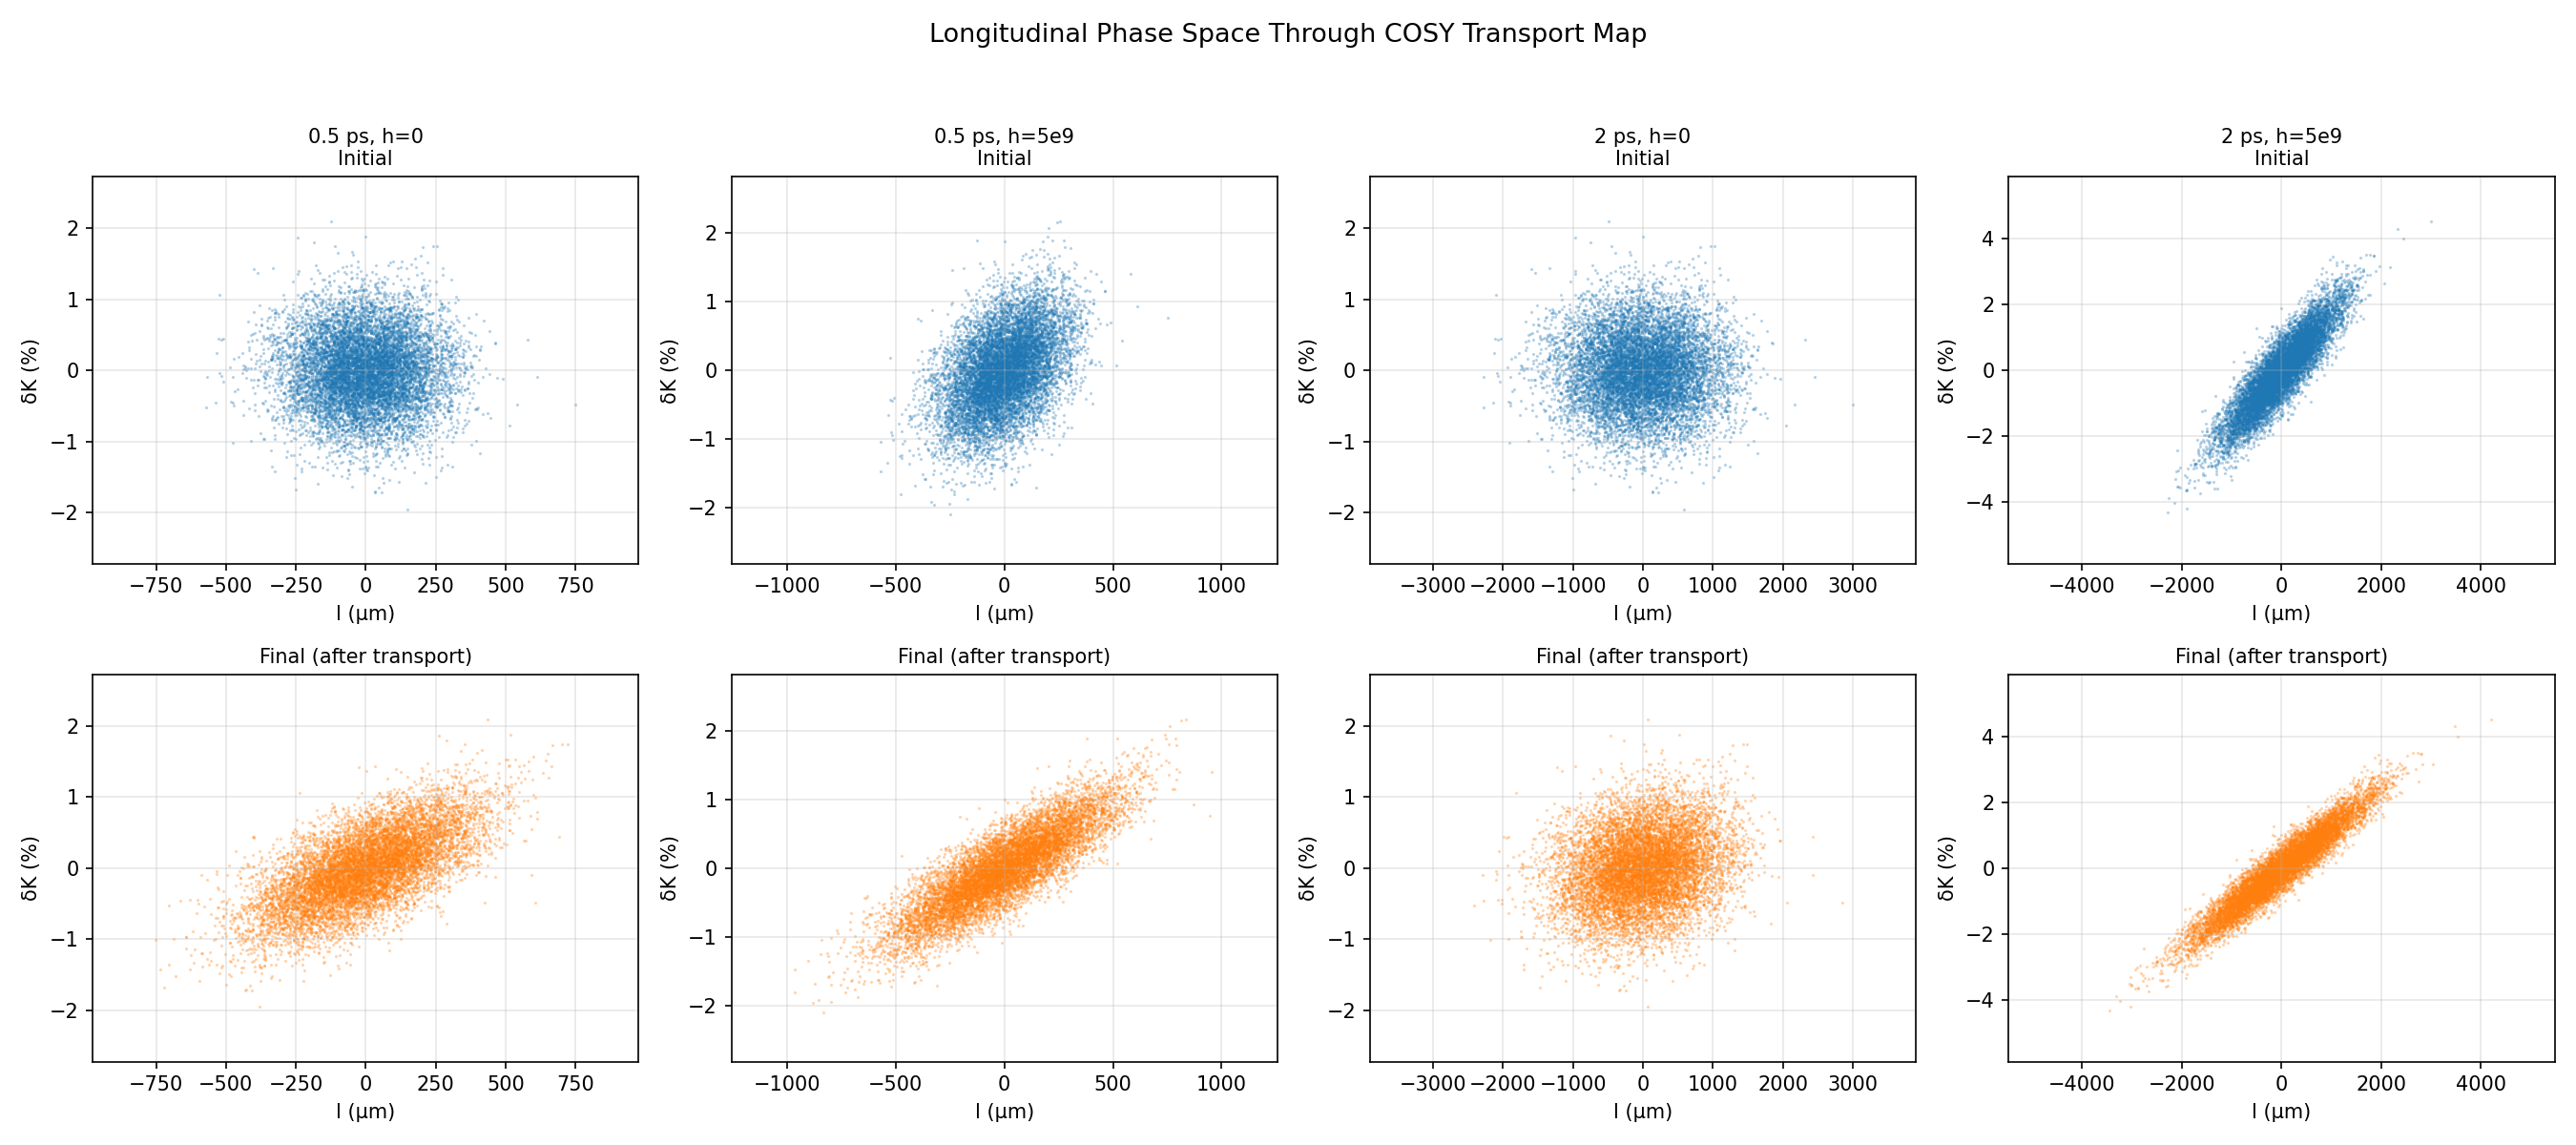
\includegraphics[width=\textwidth]{results/W9/W9_longitudinal_phase_space}
\caption{Longitudinal phase space ($l$ vs $\delta$) before (top) and
  after (bottom) transport through the COSY map.  The 0.5\,ps distributions
  broaden visibly in $l$ due to $(l|\delta)\times\sigma_\delta$ coupling;
  the 2\,ps distributions are largely unchanged.  Energy spread is
  preserved in all cases.}
\label{fig:phase-space}
\end{figure}

\begin{figure}[ht]
\centering
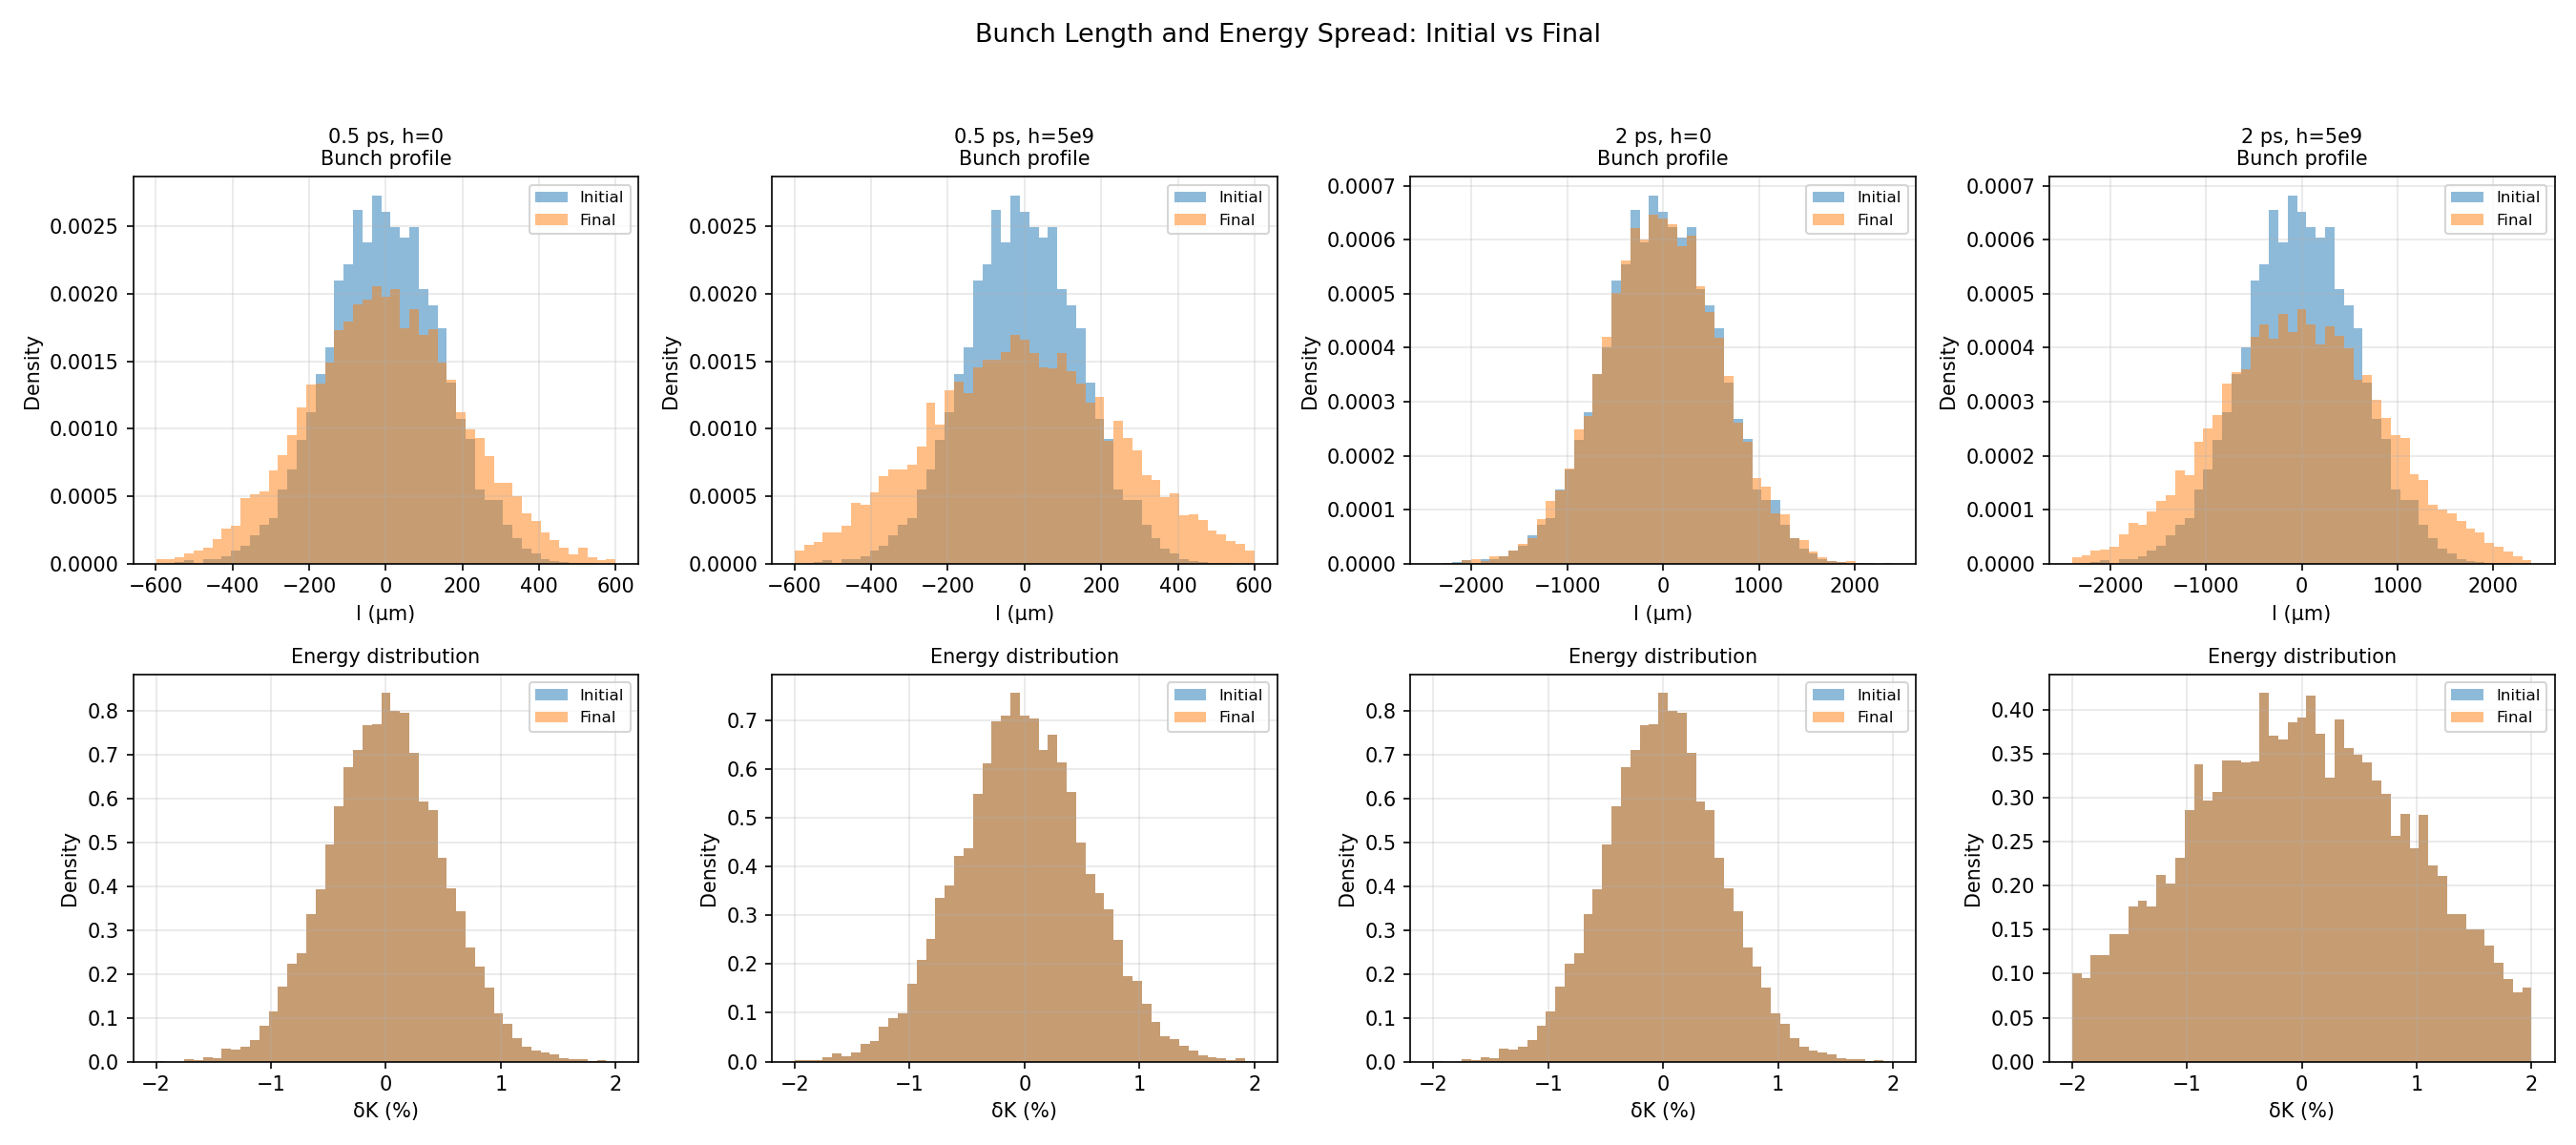
\includegraphics[width=\textwidth]{results/W9/W9_bunch_histograms}
\caption{Bunch length (top) and energy distribution (bottom) histograms:
  initial (blue) vs final (orange).  Energy distributions overlap exactly;
  bunch profiles broaden for 0.5\,ps due to chromatic path-length spread.}
\label{fig:histograms}
\end{figure}

\begin{figure}[ht]
\centering
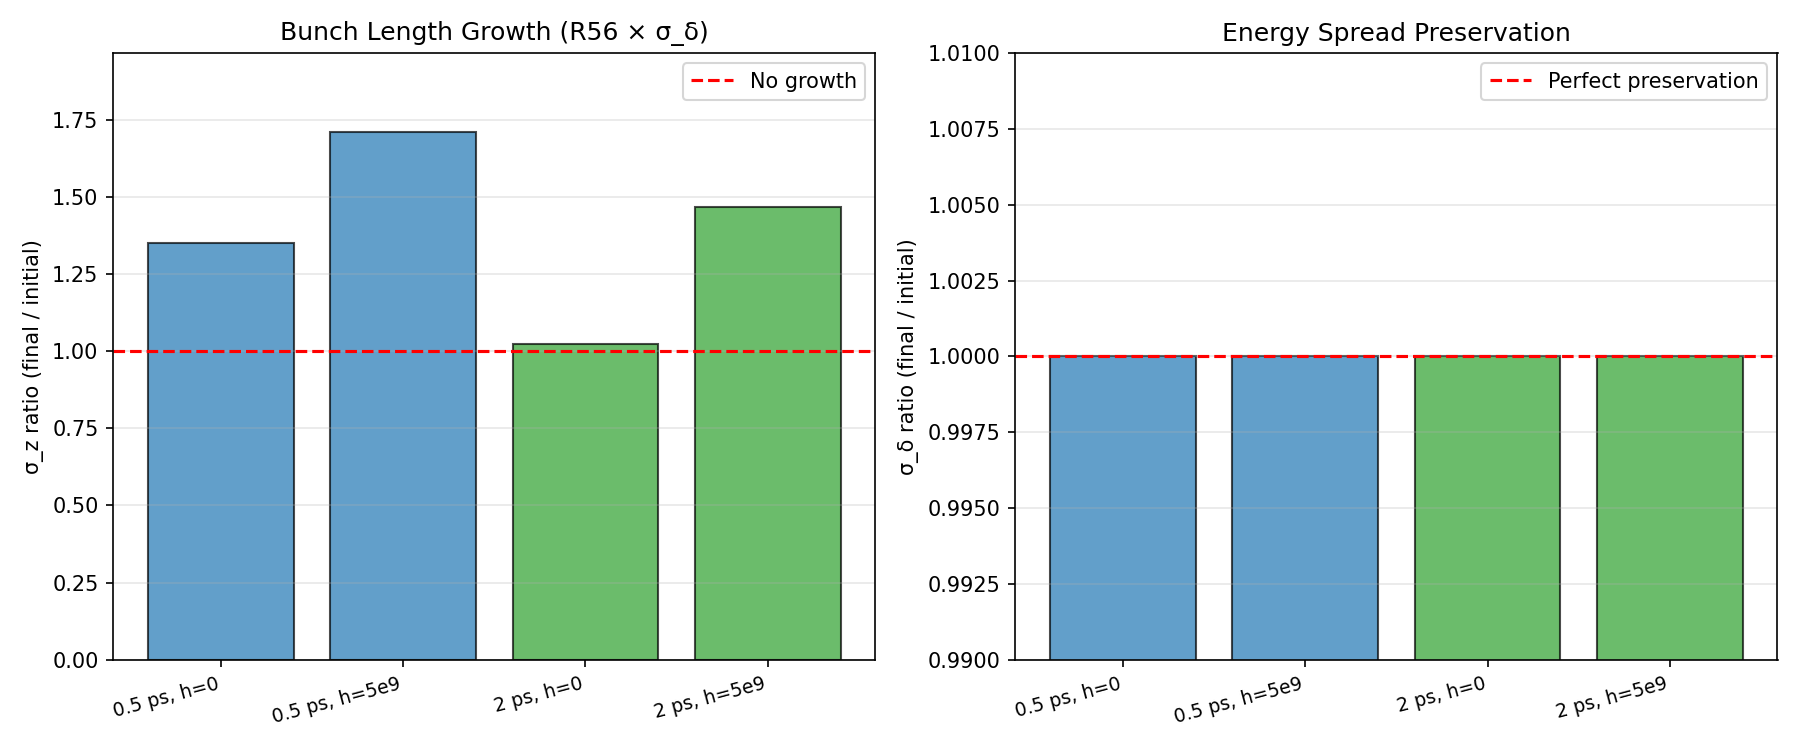
\includegraphics[width=0.85\textwidth]{results/W9/W9_preservation_ratios}
\caption{Left: bunch length growth ratio $\sigma_z^\text{out}/\sigma_z^\text{in}$.
  Right: energy spread preservation (ratio = 1.0000 for all scenarios).
  The bunch length growth arises from $(l|\delta)\times\sigma_\delta$ added in
  quadrature; it is larger for 0.5\,ps because the absolute chromatic
  contribution ($(l|\delta)\,\sigma_\delta = \SI{135}{\micro m}$) is a larger
  fraction of the initial $\sigma_z$.}
\label{fig:ratios}
\end{figure}


\subsection{$(l|\delta) = 0$ Objective}

Table~\ref{tab:r56obj} compares the baseline (transverse-only) and
augmented ($+\,(l|\delta) = 0$) optimisation results.

\begin{table}[ht]
\centering
\caption{Effect of adding $(l|\delta) = 0$ as a COSY FIT objective
  (via \texttt{ME(5,6)}).  The optimiser produces \emph{identical}
  results --- same currents, same MSE, same $(l|\delta)$.}
\label{tab:r56obj}
\begin{tabular}{@{} l S[scientific-notation=true] S[table-format=2.4] S[table-format=1.6] @{}}
\toprule
{Configuration} & {MSE} & {$(l|\delta)$ (mm)} & {Max $|\Delta I|$ (A)} \\
\midrule
Transverse only   & 2.27e-07 & 27.0890 & {---} \\
Transverse + $(l|\delta){=}0$ & 2.27e-07 & 27.0890 & 0.000000 \\
\bottomrule
\end{tabular}
\end{table}

Adding $(l|\delta) = 0$ as a FIT objective has \emph{zero effect}: the
optimiser converges to the identical solution (all 23 quad currents
unchanged, MSE unchanged, $(l|\delta)$ unchanged).  Verification with
extreme weights ($w = 100$ and $w = 10{,}000$) confirms that the
Stage~11 quadrupoles have negligible leverage over~$(l|\delta)$: at
$w = 10{,}000$, the best achievable reduction is only
\SI{9}{\micro m} (0.03\%) while transverse MSE degrades by a factor
of~2300.  The $(l|\delta)$ value is dominated by the upstream dipole
geometry and cannot be controlled by the available quad variables.


\section{Discussion}

\subsection{Bunch Lengthening Mechanism}

The dominant source of bunch lengthening is
$(l|\delta)\times\sigma_\delta$: the chromatic path-length spread
converts energy spread into longitudinal position spread.  For the
unchirped beam ($h = 0$), using transport-code notation
$R_{ij} \equiv (y_i|y_j)$:
\begin{equation}
  \sigma_{z,\text{out}}^2 \;=\; \sigma_{z,\text{in}}^2
    + R_{56}^2\,\sigma_\delta^2
    + R_{51}^2\,\sigma_x^2 + R_{52}^2\,\sigma_{x'}^2
\label{eq:sigma-z}
\end{equation}
Numerically: $R_{56}\sigma_\delta = 0.02709 \times 0.005 =
\SI{135}{\micro m}$, compared with $R_{51}\sigma_x \approx \SI{8}{\micro m}$
and $R_{52}\sigma_{x'} \approx \SI{6}{\micro m}$.  The chromatic term
dominates.

For the 0.5\,ps beam ($\sigma_z = \SI{149}{\micro m}$), adding
\SI{135}{\micro m} in quadrature gives
$\sigma_{z,\text{out}} \approx \SI{202}{\micro m}$ (ratio~1.35),
matching the simulation.  For the 2\,ps beam
($\sigma_z = \SI{596}{\micro m}$), the same absolute contribution
gives ratio~1.02 --- the longer bunch is relatively unaffected.

The chirped case adds a further stretching factor
$|1 + h\,R_{56}/(\beta c)| = |1 + 5\times10^9 \times 0.02709 / (3.0
\times10^8)| = 1.45$.  This is the dominant effect for the chirped
scenarios.

\paragraph{Implication for the 0.5\,ps mode.}
The 35\% bunch lengthening (0.5\,ps $\to$ 0.67\,ps at the undulator) is a
fixed property of the beamline geometry and the energy spread.  It does
\emph{not} affect the transverse matching and cannot be reduced by changing
quad currents (as confirmed by the $(l|\delta) = 0$ test).  Whether 0.67\,ps
is acceptable for lasing depends on the FEL gain length and slippage
requirements and is outside the scope of the transport line optimisation.

\subsection{Transverse Matching Independence}

The key result is that the $(\delta|x_j)$ map elements
($x_j \in \{x, a, y, b\}$) are all exactly zero.  This means no
transverse coordinate affects the energy deviation, so the longitudinal
subspace is decoupled from the transverse in the sense relevant to Twiss
matching.  The non-zero $(l|x_j)$ elements (path-length coupling through
bends) add path-length spread but do not feed back into the transverse
dynamics.

Consequently, the transverse Twiss match --- and therefore all 23 quad
currents --- is mathematically independent of the bunch length.  This has
now been confirmed at four independent levels:
\begin{enumerate}
  \item Analytic decoupling of the $6\times6$ transfer matrix (S9~Part~A)
  \item FELsim numerical verification at $\sigma_E = 0.5\%, 2\%, 3\%$
    (S9~Part~B1)
  \item COSY 6D DA map: $(\delta|x_j) = 0$ for all transverse $x_j$ (this
    study, Part~A)
  \item $10^4$-particle propagation: energy spread preserved exactly,
    transverse emittance growth independent of $\sigma_z$ (this study,
    Part~B)
\end{enumerate}

\subsection{Comparison with Worldwide FEL Practice}

The finding that transport line optics are independent of bunch length is
consistent with standard practice at every major FEL facility:
\begin{itemize}
  \item \textbf{LCLS:} Pulse length adjustments within the same
    compression scheme are accomplished in 1--2 minutes by changing
    linac RF phases, without transport re-optimisation~\cite{lcls-faq}.
  \item \textbf{SACLA:} Two beamlines (BL2, BL3) simultaneously receive
    beams with different bunch lengths pulse-by-pulse, achieved by RF
    phase modulation alone~\cite{Tono2019}.
  \item \textbf{FERMI:} Compression factor varied experimentally while
    keeping chicane geometry, dipole angles, and beam energy
    constant~\cite{DiMitri2012}.
  \item \textbf{SPARC:} Velocity bunching in the first linac section
    demonstrated compression ratios up to $C = 14$ with emittance
    compensation~\cite{Ferrario2010}.
  \item \textbf{CLARA:} Designed from the outset for dual-mode operation
    (standard acceleration and velocity bunching) using the same
    S-band linac~\cite{Snedden2024}.
\end{itemize}

\subsection{Recommended 2\,ps $\to$ 0.5\,ps Switching Procedure}

The 0.5\,ps operating mode requires changing \emph{only} the injector/RF
settings upstream of the transport line entrance.  The recommended approach
for the UH MkV is velocity bunching: shifting the first S-band linac
section phase from on-crest to $\sim$30--60$^\circ$ off-crest, compressing
the bunch while simultaneously accelerating it.  This avoids the need
for a dedicated magnetic bunch compressor and the associated CSR-induced
emittance growth.

The FC1 chicane in the existing transport line is not suitable for
compression: its $(l|\delta) \approx \SI{-3}{mm}$ (from the chicane alone) is
too small.  Achieving $C = 4$ via the chicane would require
$h > 5\times10^{10}$\,s$^{-1}$, increasing $\sigma_\delta$ to $>$10\% ---
far beyond the energy acceptance of the downstream optics.


\section{Summary}

\begin{enumerate}
  \item The full 6D COSY INFINITY transfer map confirms that the
    transverse-longitudinal coupling is zero in the Twiss-matching sense:
    $(\delta|x_j) = 0$ for all transverse $x_j$ (Table~\ref{tab:map}).
  \item Transport line $(l|\delta) = \SI{27.09}{mm}$ (full line) and
    $(l|\delta\delta) = 0$.  The non-zero $(l|\delta)$ causes bunch
    lengthening (35\% for 0.5\,ps, 2.5\% for 2\,ps at
    $\sigma_\delta = 0.5\%$), but this is a fixed property of the dipole
    geometry and does not affect the transverse matching
    (Table~\ref{tab:bunch}, Fig.~\ref{fig:ratios}).
  \item Adding $(l|\delta) = 0$ as a FIT objective produces an
    \emph{identical} solution --- zero change in all 23 quad currents
    and in the MSE (Table~\ref{tab:r56obj}).
  \item The 2\,ps $\to$ 0.5\,ps switch requires only injector RF phase
    changes (velocity bunching).  All transport line settings remain
    identical.  This is standard practice at LCLS, SACLA, FERMI, SPARC,
    CLARA, SwissFEL, and the European~XFEL\@.
\end{enumerate}


\begin{thebibliography}{9}
\bibitem{weinberg2025}
  M.~Weinberg, A.~Fisher, and R.~Li,
  ``Design of the UH Mark V Free Electron Laser,''
  arXiv:2510.14061v1, Table~I.

\bibitem{Ferrario2010}
  M.~Ferrario \textit{et al.},
  ``Experimental Demonstration of Emittance Compensation with
  Velocity Bunching,''
  Phys.\ Rev.\ Lett.\ \textbf{104}, 054801 (2010).

\bibitem{DiMitri2012}
  S.~Di~Mitri \textit{et al.},
  ``Coherent synchrotron radiation and microbunching in bunch
  compressors and free-electron lasers,''
  Phys.\ Rev.\ ST Accel.\ Beams \textbf{15}, 020701 (2012).

\bibitem{Tono2019}
  K.~Tono, T.~Hara, M.~Yabashi, and H.~Tanaka,
  ``Multiple-beamline operation of SACLA,''
  J.\ Synchrotron Rad.\ \textbf{26}, 595--602 (2019).

\bibitem{Snedden2024}
  E.~W.~Snedden \textit{et al.},
  ``Specification and design for full energy beam exploitation of the
  compact linear accelerator for research and applications,''
  Phys.\ Rev.\ Accel.\ Beams \textbf{27}, 041602 (2024).

\bibitem{lcls-faq}
  SLAC National Accelerator Laboratory,
  ``LCLS Machine FAQ,''
  \url{https://lcls.slac.stanford.edu/machine/faq}.
\end{thebibliography}

\end{document}
